\documentclass[11pt]{article}

\usepackage[margin=1in]{geometry}
\usepackage{amsmath, amssymb, amsthm}
\usepackage{tikz}
\usetikzlibrary{arrows.meta, positioning, fit, backgrounds, calc,
                decorations.pathmorphing, decorations.markings,
                shapes.geometric}
\usepackage{float}
\usepackage{array}
\usepackage{booktabs}
\usepackage{tcolorbox}
\tcbuselibrary{skins, breakable}
\usepackage{xcolor}
\usepackage{enumitem}
\usepackage{hyperref}
\hypersetup{colorlinks=true, linkcolor=blue!55!black, urlcolor=blue!55!black}

\definecolor{accent}{RGB}{30,90,160}
\definecolor{accent2}{RGB}{170,60,30}
\definecolor{accent3}{RGB}{40,130,80}
\definecolor{accent4}{RGB}{120,70,150}
\definecolor{soft}{RGB}{238,243,250}
\definecolor{soft2}{RGB}{250,243,236}
\definecolor{soft3}{RGB}{238,248,242}
\definecolor{soft4}{RGB}{245,240,250}

\newtcolorbox{keybox}[1]{
  colback=soft, colframe=accent, fonttitle=\bfseries,
  title={#1}, breakable, boxrule=0.6pt, arc=2pt, left=6pt, right=6pt}

\newtcolorbox{watchbox}[1]{
  colback=soft2, colframe=accent2, fonttitle=\bfseries,
  title={#1}, breakable, boxrule=0.6pt, arc=2pt, left=6pt, right=6pt}

\newtcolorbox{examplebox}[1]{
  colback=soft3, colframe=accent3, fonttitle=\bfseries,
  title={#1}, breakable, boxrule=0.6pt, arc=2pt, left=6pt, right=6pt}

\newtcolorbox{intuitionbox}[1]{
  colback=soft4, colframe=accent4, fonttitle=\bfseries,
  title={#1}, breakable, boxrule=0.6pt, arc=2pt, left=6pt, right=6pt}

\title{\textbf{Mann \S3.2 -- \S3.5}\\[2pt]
\Large Lie Groups, Algebras, $SO(3)$, and the Appendix\\[4pt]
\large A Slow, Heavily Annotated Walkthrough}
\author{Reading companion --- Mann, \emph{An Introduction to Particle Physics
and the Standard Model}, Ch.~3}
\date{2026--05--20}

\begin{document}
\maketitle

\begin{intuitionbox}{Before you start: the big picture}
Chapter~3 has been climbing a ladder:
\begin{itemize}[leftmargin=1.5em, itemsep=2pt]
  \item \S3.1.1 --- what a \emph{group} is (abstract symbols + a rule).
  \item \S3.1.2 --- a \emph{representation} turns those symbols into matrices.
  \item \S3.1.3 --- \emph{irreducible} reps are the atomic building blocks.
  \item \S3.1.4 --- finite groups can be written as a multiplication table.
\end{itemize}
\textbf{Now the chapter pivots.} Most symmetries in physics --- rotations,
phase rotations, Lorentz boosts --- have \emph{infinitely many} elements.
You can't write down a multiplication table with an uncountable number of
rows. So \S3.2--\S3.5 build the machinery that handles continuous symmetries:
\begin{enumerate}[leftmargin=1.5em, itemsep=2pt]
  \item \textbf{\S3.2 Lie groups} --- smooth, continuous groups (rotations,
    etc.) and the idea that they are completely described by a small finite
    set of \emph{generators}.
  \item \textbf{\S3.3 Algebras} --- a more relaxed structure than a group:
    just a vector space with a way to combine vectors.
  \item \textbf{\S3.3.1 Lie algebras} --- the algebra you get by zooming in
    on a Lie group at the identity. This is the central computational
    object.
  \item \textbf{\S3.4 $SO(3)$} --- one full worked example: rotations in
    3D, end to end.
  \item \textbf{\S3.5 Appendix} --- the proof that closure of the Lie
    group $\Rightarrow$ the commutator relation of the Lie algebra.
\end{enumerate}
The payoff: \emph{instead of studying an infinite curved manifold of group
elements, you only have to study a finite-dimensional vector space and the
commutators of its basis vectors.} That replacement is what makes Lie
theory tractable, and it is the central technical idea of the rest of the
book.
\end{intuitionbox}

%==============================================================
\section{\S3.2 --- Lie Groups}
%==============================================================

\subsection*{What's new compared to finite groups}

A \emph{finite} group has a discrete list of elements: $\{e, g_1, g_2,
\ldots, g_n\}$. A \emph{Lie group} is a group whose elements depend
\emph{smoothly} on some continuous knobs $\theta^a$.

\begin{intuitionbox}{Two pictures to keep in your head}
\begin{itemize}[leftmargin=1.5em, itemsep=4pt]
  \item \textbf{Discrete (finite) group} -- imagine a row of separated
    beads. You can only sit on a bead.  Going from one bead to another
    is a discrete jump.
  \item \textbf{Lie group} -- imagine a smooth curve, surface, or
    higher-dimensional sheet (a ``manifold''). Every point on the sheet
    is a group element, and you can slide continuously between them.
    Group multiplication is a smooth function of where you are on the
    sheet.
\end{itemize}
\end{intuitionbox}

\begin{figure}[H]
\centering
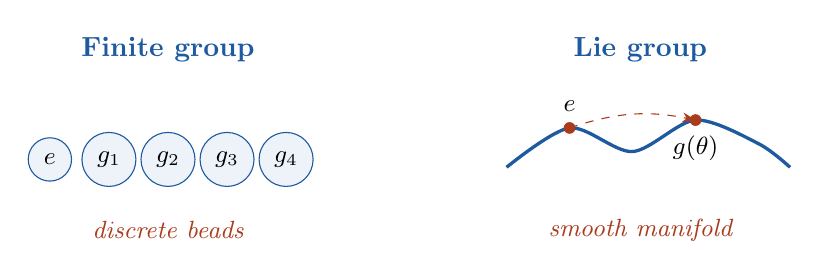
\begin{tikzpicture}[font=\sffamily]
  % left: discrete
  \begin{scope}[xshift=0cm]
    \node[accent, font=\bfseries] at (1.5, 1.4) {Finite group};
    \foreach \x/\lab in {0/$e$, 0.75/$g_1$, 1.5/$g_2$, 2.25/$g_3$, 3.0/$g_4$} {
      \node[circle, draw=accent, fill=soft, minimum size=0.55cm,
            font=\small] at (\x, 0) {\lab};
    }
    \node[accent2, font=\itshape\small] at (1.5, -0.9)
      {discrete beads};
  \end{scope}
  % right: smooth curve
  \begin{scope}[xshift=6cm]
    \node[accent, font=\bfseries] at (1.5, 1.4) {Lie group};
    \draw[accent, very thick, decoration={zigzag, segment length=0pt,
          amplitude=0pt}] plot[smooth] coordinates
      {(-0.2,-0.1) (0.6,0.4) (1.4,0.1) (2.2,0.5) (3.0,0.2) (3.4,-0.1)};
    \node[circle, fill=accent2, inner sep=1.5pt, label=above:{\small $e$}]
      at (0.6, 0.4) {};
    \node[circle, fill=accent2, inner sep=1.5pt,
          label=below:{\small $g(\theta)$}] at (2.2, 0.5) {};
    \draw[-Stealth, accent2, dashed] (0.6,0.4) to[bend left=15] (2.2,0.5);
    \node[accent2, font=\itshape\small] at (1.5, -0.9)
      {smooth manifold};
  \end{scope}
\end{tikzpicture}
\caption{Finite group vs.\ Lie group. In the Lie group every point on the
smooth curve is a separate group element; the parameter $\theta$ tells
you where you are.}
\end{figure}

\subsection*{Mann's defining formula, decoded slowly}

Mann writes a typical Lie group element as
\begin{equation}
  g \;=\; g(\theta^1, \ldots, \theta^N) \;=\;
  \exp\!\left[\, i\, \theta^a\, T_a \,\right]
  \;=\; \exp\!\left[\, i \vec\theta \cdot \vec T \,\right].
  \tag{3.1}
\end{equation}
This formula is dense. Let's take it one symbol at a time.

\begin{keybox}{Reading equation (3.1) piece by piece}
\begin{description}[style=nextline, leftmargin=0pt, itemsep=4pt]
  \item[$\theta^1, \ldots, \theta^N$] are continuous real \emph{parameters} ---
    the ``knobs'' you can turn. The number $N$ is fixed by the group
    (for $SO(3)$, $N=3$, one knob per rotation axis).
  \item[$T_a$, $a = 1,\ldots,N$] are fixed matrices (or operators) called
    \textbf{generators}. There are exactly $N$ of them, one per knob.
  \item[$\theta^a T_a$] uses the Einstein summation convention:
    $\theta^a T_a = \theta^1 T_1 + \theta^2 T_2 + \cdots + \theta^N T_N$.
    Repeated indices are summed.
  \item[$i$] is the imaginary unit. The $i$ is a physics convention that
    makes the $T_a$ Hermitian (so they correspond to observables, e.g.\
    angular-momentum components).
  \item[{$\exp[\,\cdot\,]$}] is the \textbf{matrix exponential},
    defined by its power series:
    \[ \exp[M] = I + M + \tfrac{1}{2!} M^2 + \tfrac{1}{3!} M^3 + \cdots \]
    For an ordinary number this is the usual exponential; for a matrix
    it produces another matrix.
\end{description}
\end{keybox}

\begin{intuitionbox}{Why this is amazing}
A continuous group has \emph{infinitely many} elements (every value of
every $\theta^a$ gives a different one). But equation~(3.1) says all of
them can be built out of a small fixed list of $N$ matrices, the $T_a$.
Know the $N$ generators, know the whole group.

Compare:
\begin{itemize}[leftmargin=1.5em, itemsep=2pt]
  \item Finite group of order $n$: $n$ entries in a multiplication table.
  \item Lie group: \emph{infinitely many} elements, but only $N$
    generators (often $N \leq 10$) needed to encode them.
\end{itemize}
That's an enormous compression of information.
\end{intuitionbox}

\subsection*{What ``generator'' means geometrically}

Think of the Lie group as a curved surface (manifold). The identity
element $e$ corresponds to the origin (all $\theta^a = 0$). The
generators $T_a$ are like \emph{tangent vectors at the identity}: they
tell you which way you start moving when you turn the $a^{\text{th}}$
knob slightly.

\begin{figure}[H]
\centering
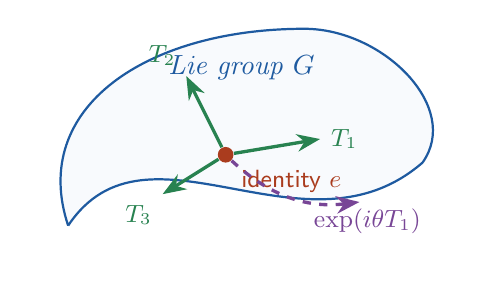
\begin{tikzpicture}[font=\sffamily]
  % surface (a curved patch)
  \draw[accent, thick, fill=soft, fill opacity=0.4]
    (0,0) .. controls (1,1.5) and (3,-0.5) .. (4.5,0.8)
          .. controls (5,1.5) and (4,2.5) .. (3,2.5)
          .. controls (1,2.5) and (-0.5,1.5) .. (0,0);
  \node[accent, font=\itshape] at (2.2, 2.0) {Lie group $G$};
  % identity point
  \node[circle, fill=accent2, inner sep=2pt,
        label={[accent2]below right:\small identity $e$}]
    (e) at (2.0, 0.9) {};
  % tangent vectors at identity
  \draw[-Stealth, accent3, very thick] (e) -- ++(1.2, 0.2)
    node[right, accent3] {\small $T_1$};
  \draw[-Stealth, accent3, very thick] (e) -- ++(-0.5, 1.0)
    node[above left, accent3] {\small $T_2$};
  \draw[-Stealth, accent3, very thick] (e) -- ++(-0.8, -0.5)
    node[below left, accent3] {\small $T_3$};
  % a curve through e
  \draw[accent4, dashed, very thick, -Stealth]
    (e) to[bend right=25] (3.7, 0.3);
  \node[accent4, font=\small] at (3.8, 0.05)
    {$\exp(i\theta T_1)$};
\end{tikzpicture}
\caption{Geometrical picture. The generators $T_a$ are tangent vectors at
the identity. The exponential map $\exp(i\theta^a T_a)$ takes you
\emph{along} the manifold, tracing out an actual group element. The
curved arrow shows the curve generated by turning only the $T_1$ knob.}
\end{figure}

\begin{watchbox}{Footnote (\dag\dag): a subtle caveat}
Mann's footnote: the generators contain all the \emph{local} information
about the group, i.e.\ they reconstruct every element \emph{continuously
connected to the identity}. Some groups have ``disconnected pieces''
(e.g.\ the orthogonal group $O(3)$ contains rotations \emph{and}
reflections; you can't continuously deform a rotation into a reflection).
The generators only describe the piece containing the identity. The
disconnected pieces matter in certain QED contexts (vacuum structure;
ch.~25) but not for the bulk of particle physics.
\end{watchbox}

\subsection*{Why Lie groups dominate physics}

Most physical symmetries are \emph{continuous}: you can rotate by any
real angle, boost by any real velocity, multiply a wavefunction by any
real phase. Mann gives the high-level taxonomy:

\begin{itemize}[leftmargin=1.5em, itemsep=2pt]
  \item \textbf{Spacetime symmetries} act on the spacetime coordinates
    $(t, x, y, z)$. Examples: rotations $SO(3)$, Lorentz boosts $SO(3,1)$.
  \item \textbf{Internal symmetries} act on wavefunction components or
    on charges, leaving coordinates alone. Examples: $U(1)$ phase
    rotation in electromagnetism, $SU(3)$ color in QCD, $SU(2)$ weak
    isospin.
\end{itemize}

A streamlined version of Mann's Table~3.4 (the catalog of Lie groups you
will meet again and again in this book):

\begin{table}[H]
\centering
\renewcommand{\arraystretch}{1.2}
\begin{tabular}{@{}lll@{}}
\toprule
\textbf{Group} & \textbf{Defining property} & \textbf{Where it shows up} \\
\midrule
$U(n)$    & $n\times n$ unitary $(U^\dagger U = I)$
          & $U(1)$: electromagnetism \\
$SU(n)$   & $U(n)$ with $\det U = 1$
          & $SU(3)$: strong, $SU(2)$: weak \\
$O(n)$    & $n\times n$ orthogonal $(O^TO = I)$
          & $O(3)$: rotations + reflections \\
$SO(n)$   & $O(n)$ with $\det O = 1$
          & $SO(3)$: rotations, $SO(3,1)$: Lorentz \\
$Sp(n)$   & $n\times n$ symplectic
          & phase-space structure (Hamilton'n mech) \\
\bottomrule
\end{tabular}
\caption{The standard Lie groups that organize particle physics. The
``$S$'' in $SO$ / $SU$ stands for ``special'' and means $\det = 1$.}
\end{table}

\begin{intuitionbox}{Etymology cheat-sheet}
\begin{itemize}[leftmargin=1.5em, itemsep=2pt]
  \item $U$ = \textbf{Unitary} (preserves complex inner product;
    equivalent to: preserves probability).
  \item $O$ = \textbf{Orthogonal} (preserves real inner product;
    equivalent to: preserves lengths and angles).
  \item $S$ = \textbf{Special} (the additional restriction
    $\det = +1$; rules out reflections / orientation-flips).
  \item $Sp$ = \textbf{Symplectic} (preserves a specific antisymmetric
    form; the language of Hamiltonian mechanics).
\end{itemize}
\end{intuitionbox}

%==============================================================
\section{\S3.3 --- Algebras}
%==============================================================

\subsection*{What an algebra is (and isn't)}

An \textbf{algebra} is a more \emph{relaxed} structure than a group:
\begin{itemize}[leftmargin=1.5em, itemsep=2pt]
  \item Start with a vector space $V$ (so addition and scalar
    multiplication work the usual way).
  \item Add a binary ``combining'' operation $\circ$ that takes two
    vectors and produces a third \emph{still in $V$}.
\end{itemize}
That's it. \textbf{An algebra does not require an identity element. It
does not require inverses.} It only requires \emph{closure} (the result
stays in the space).

\begin{equation}
  v_I \circ v_J \;=\; \sum_K C^{IJ}_{\;\;\;K}\, v_K \;=\; C^{IJ}_{\;\;\;K}\, v_K
  \tag{3.2}
\end{equation}

\begin{keybox}{What equation (3.2) is really saying}
Pick any two basis vectors $v_I$ and $v_J$. Combine them with $\circ$.
The result, being still in the vector space $V$, can be written as a
linear combination of the basis vectors $v_K$. The coefficients of that
combination, $C^{IJ}_{\;\;\;K}$, are called the \textbf{structure
constants}. They are just numbers, and they tell you \emph{everything}
about how the algebra combines. Know the structure constants, know the
algebra.
\end{keybox}

\begin{examplebox}{Concrete example: the vector cross product}
Take $V$ = vectors in 3D, with basis $\{\hat x, \hat y, \hat z\}$, and
combining operation $\circ$ = $\times$ (the cross product). Then
\[
  \hat x \times \hat y = \hat z, \qquad
  \hat y \times \hat z = \hat x, \qquad
  \hat z \times \hat x = \hat y,
\]
with all other cross products either zero or sign-flipped. This gives
the structure constants $C^{IJ}_{\;\;\;K} = \epsilon_{IJK}$, the
Levi-Civita symbol. So \emph{3D vector-cross-product space is an
algebra} --- and a particularly important one, because we'll see
shortly that it's the same algebra as the rotation group's.
\end{examplebox}

\begin{intuitionbox}{Group vs.\ algebra in one line}
\begin{description}[style=nextline, leftmargin=0pt, itemsep=3pt]
  \item[\textbf{Group:}] closure + associativity + identity + inverses.
  \item[\textbf{Algebra:}] vector space + closure under $\circ$.
\end{description}
An algebra is what you keep when you throw away identities, inverses,
and associativity-as-a-requirement, and keep just the rule for combining
two things into a third. It is a \emph{leaner} structure than a group.
\end{intuitionbox}

%==============================================================
\subsection*{\S3.3.1 --- Lie Algebras}
%==============================================================

\subsubsection*{The bridge: zooming in on a Lie group}

Here is the central move of the whole chapter.

\begin{intuitionbox}{The key idea}
A Lie group is a curved manifold. If you stand at the identity and
\emph{zoom in close enough}, the manifold looks flat --- like a vector
space. That tangent vector space, equipped with the right combining
operation, is a \textbf{Lie algebra}. The Lie algebra is, in effect,
the \textbf{linearization} of the Lie group near its identity.

Why bother? Because vector spaces are radically easier to work with than
curved manifolds. By passing to the Lie algebra you replace nonlinear
multiplication of group elements with \emph{linear} algebra on a finite
set of basis vectors.
\end{intuitionbox}

The basis vectors of the Lie algebra turn out to be exactly the
generators $T_a$ we already met in equation~(3.1). The combining
operation is the \textbf{commutator}:
\begin{equation}
  [T^a, T^b] \;\equiv\; T^a T^b - T^b T^a \;=\; i f^{abc}\, T^c
  \tag{3.3}
\end{equation}

Reading this slowly:
\begin{itemize}[leftmargin=1.5em, itemsep=3pt]
  \item $[T^a, T^b]$ is the \emph{commutator} of two generators. It
    measures the failure of $T^a$ and $T^b$ to commute under
    multiplication.
  \item The right-hand side $i f^{abc} T^c$ says: \emph{the commutator
    is itself a linear combination of generators}. So the algebra is
    closed under the commutator (which is what makes it an algebra in
    the sense of \S3.3).
  \item $f^{abc}$ are the \textbf{structure constants} of the Lie
    algebra (the $C^{IJ}_{\;\;K}$ of the previous section, specialized
    to this context). They are just numbers --- but they completely
    encode the local geometry of the Lie group.
\end{itemize}

\begin{keybox}{Jacobi identity}
The associativity of group multiplication translates into a constraint
on commutators:
\begin{equation}
  \big[\,[T^a, T^b],\, T^c\,\big] + \big[\,[T^b, T^c],\, T^a\,\big] +
  \big[\,[T^c, T^a],\, T^b\,\big] \;=\; 0
  \tag{3.4}
\end{equation}
This is the \textbf{Jacobi identity}. Any vector space equipped with a
bracket $[\cdot,\cdot]$ that is antisymmetric \emph{and} obeys (3.4) is
called a Lie algebra. The Jacobi identity is the algebra-level remnant
of group associativity.
\end{keybox}

\begin{intuitionbox}{The whole point of Lie algebras, in two sentences}
A Lie group's curved geometry is hard. Its Lie algebra is just a
finite-dimensional vector space with a bracket, which is linear algebra
--- and linear algebra is something we can compute with. \emph{Almost
every calculation in particle physics symmetry is done at the Lie
algebra level, not the Lie group level.}
\end{intuitionbox}

%==============================================================
\section{\S3.4 --- Worked Example: the Rotation Group $SO(3)$}
%==============================================================

Now we do all of the above for one specific group, end to end. This is
the most important worked example in the chapter --- if you understand
this section, you understand the rest.

\subsection*{Step 1: write down rotations as matrices}

A rotation by angle $\theta$ about the $\hat z$-axis sends
\[
  x' = \cos\theta\, x + \sin\theta\, y, \qquad
  y' = -\sin\theta\, x + \cos\theta\, y, \qquad
  z' = z.
\]
In matrix form,
\[
  R_z(\theta) = \begin{pmatrix} \cos\theta & \sin\theta & 0 \\
                                -\sin\theta & \cos\theta & 0 \\
                                0 & 0 & 1 \end{pmatrix}.
\]
Similarly $R_x(\theta_x)$ and $R_y(\theta_y)$ are defined by rotations
about $\hat x$ and $\hat y$. The full set of 3D rotations is what you
get by multiplying these together with arbitrary $\theta_x, \theta_y,
\theta_z$. This set is the group $SO(3)$ --- $3\times3$ orthogonal
matrices with $\det = +1$.

\begin{figure}[H]
\centering
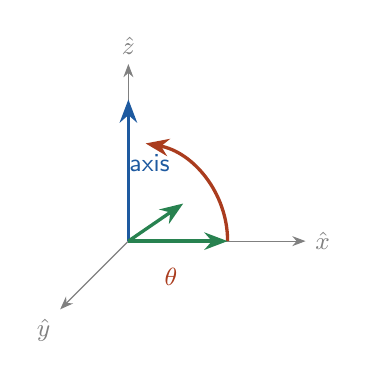
\begin{tikzpicture}[font=\sffamily, scale=0.9]
  % axes
  \draw[-Stealth, gray] (0,0,0) -- (2.5,0,0) node[right]{\small $\hat x$};
  \draw[-Stealth, gray] (0,0,0) -- (0,2.5,0) node[above]{\small $\hat z$};
  \draw[-Stealth, gray] (0,0,0) -- (0,0,2.5) node[below left]{\small $\hat y$};
  % rotation about z
  \draw[-Stealth, accent2, very thick] (1.4,0,0) arc[start angle=0,
        end angle=80, radius=1.4];
  \node[accent2] at (1.1, 0.0, 1.3) {\small $\theta$};
  % the rotation axis highlighted
  \draw[accent, very thick, -Stealth] (0,0,0) -- (0,2.0,0);
  \node[accent] at (0.3, 1.1, 0) {\small axis};
  % the rotated vector
  \draw[-Stealth, accent3, very thick] (0,0,0) -- (1.4,0,0);
  \draw[-Stealth, accent3, very thick] (0,0,0) --
    ({1.4*cos(80)},0,{-1.4*sin(80)});
\end{tikzpicture}
\caption{A rotation about the $\hat z$-axis through angle $\theta$. The
parameter $\theta$ can be any real number; for each value you get a
different element of $SO(3)$.}
\end{figure}

\subsection*{Step 2: zoom in near the identity to extract a generator}

The identity element of $SO(3)$ is no rotation: $\theta = 0$. Near
$\theta = 0$ we Taylor-expand $\cos\theta \approx 1$, $\sin\theta
\approx \theta$:
\[
  R_z(\theta) \;\approx\; \begin{pmatrix} 1 & \theta & 0 \\
                                          -\theta & 1 & 0 \\
                                          0 & 0 & 1 \end{pmatrix}
  \;=\; I \;+\; \theta \begin{pmatrix} 0 & 1 & 0 \\
                                       -1 & 0 & 0 \\
                                       0 & 0 & 0 \end{pmatrix}.
\]
Mann wants the convention $R_z \approx I + i \theta T_z$, so we read off
\begin{equation}
  T_z \;=\; -i \begin{pmatrix} 0 & 1 & 0 \\
                               -1 & 0 & 0 \\
                               0 & 0 & 0 \end{pmatrix}.
\end{equation}
That extra $-i$ is bookkeeping: it makes $T_z$ \emph{Hermitian}, so it
deserves to be called a physical generator (its eigenvalues are real,
just like an observable).

Repeating the same exercise for $R_x$ and $R_y$ gives the three
generators of $SO(3)$:
\[
  T_x = -i\begin{pmatrix} 0 & 0 & 0 \\ 0 & 0 & 1 \\
                          0 & -1 & 0 \end{pmatrix},
  \quad
  T_y = -i\begin{pmatrix} 0 & 0 & -1 \\ 0 & 0 & 0 \\
                          1 & 0 & 0 \end{pmatrix},
  \quad
  T_z = -i\begin{pmatrix} 0 & 1 & 0 \\ -1 & 0 & 0 \\
                          0 & 0 & 0 \end{pmatrix}.
\]
These three matrices are a \emph{basis} for the Lie algebra
$\mathfrak{so}(3)$.

\begin{intuitionbox}{Why three?}
The dimension of the Lie algebra equals the number of independent
parameters of the Lie group. $SO(3)$ has three (one rotation angle per
axis: $\theta_x, \theta_y, \theta_z$). So $\mathfrak{so}(3)$ has three
basis vectors. In general, an $N$-parameter Lie group has an
$N$-dimensional Lie algebra.
\end{intuitionbox}

\subsection*{Step 3: compute a commutator (the hard step, fully shown)}

We want to verify $[T_x, T_y] = i T_z$. Just plug in. With
$(-i)^2 = -1$:
\begin{align*}
  T_x T_y &= (-i)^2
    \begin{pmatrix} 0 & 0 & 0 \\ 0 & 0 & 1 \\ 0 & -1 & 0 \end{pmatrix}
    \begin{pmatrix} 0 & 0 & -1 \\ 0 & 0 & 0 \\ 1 & 0 & 0 \end{pmatrix}
    \;=\; -\begin{pmatrix} 0 & 0 & 0 \\ 1 & 0 & 0 \\ 0 & 0 & 0 \end{pmatrix},
\\[4pt]
  T_y T_x &= (-i)^2
    \begin{pmatrix} 0 & 0 & -1 \\ 0 & 0 & 0 \\ 1 & 0 & 0 \end{pmatrix}
    \begin{pmatrix} 0 & 0 & 0 \\ 0 & 0 & 1 \\ 0 & -1 & 0 \end{pmatrix}
    \;=\; -\begin{pmatrix} 0 & 1 & 0 \\ 0 & 0 & 0 \\ 0 & 0 & 0 \end{pmatrix}.
\end{align*}
Subtracting:
\[
  [T_x, T_y] = T_x T_y - T_y T_x
  = -\begin{pmatrix} 0 & 0 & 0 \\ 1 & 0 & 0 \\ 0 & 0 & 0 \end{pmatrix}
    +\begin{pmatrix} 0 & 1 & 0 \\ 0 & 0 & 0 \\ 0 & 0 & 0 \end{pmatrix}
  = \begin{pmatrix} 0 & 1 & 0 \\ -1 & 0 & 0 \\ 0 & 0 & 0 \end{pmatrix}.
\]
And $i T_z = i \cdot (-i)\begin{pmatrix} 0 & 1 & 0 \\ -1 & 0 & 0 \\
0 & 0 & 0 \end{pmatrix} = \begin{pmatrix} 0 & 1 & 0 \\ -1 & 0 & 0 \\
0 & 0 & 0 \end{pmatrix}$. They match. So $[T_x, T_y] = i T_z$.

By symmetry the other two commutators come out $[T_y, T_z] = i T_x$ and
$[T_z, T_x] = i T_y$. All three can be packaged into the single formula
\begin{equation}
  [T^a, T^b] \;=\; i\, \epsilon^{abc}\, T^c
  \tag{3.10}
\end{equation}
where the structure constants $f^{abc} = \epsilon^{abc}$ are exactly the
Levi-Civita symbol from the cross-product example earlier in \S3.3.
\textbf{The Lie algebra $\mathfrak{so}(3)$ has the same structure
constants as the 3D vector cross product.} That is not a coincidence:
infinitesimal rotations \emph{are} cross products with the rotation
axis.

\subsection*{Step 4: convention --- rename $T_a \to J_a$}

The algebra $\mathfrak{so}(3)$ and the group $SO(3)$ are so ubiquitous
in physics --- they are the angular momentum algebra you saw in quantum
mechanics --- that the generators get a special name:
\[
  T_a \;\longrightarrow\; J_a, \qquad [J^a, J^b] \;=\; i\,\epsilon^{abc} J^c.
  \tag{3.13}
\]
These are the angular momentum operators. The hydrogen-atom commutation
relations $[J_x, J_y] = i\hbar J_z$ (with $\hbar = 1$ in natural units)
are literally this equation.

\subsection*{Step 5: exponentiate back to recover a finite rotation}

The exponential map walks you from the algebra back to the group. With
$\vec\theta = \theta \hat y$:
\[
  \exp(i\theta J_y)
  = I + (i\theta J_y) + \tfrac{1}{2!}(i\theta J_y)^2 + \cdots
\]
Mann grinds through the series; the trigonometric pattern emerges
because $J_y^2$ acts as a projector that eats only the $x,z$ subspace.
The final result is
\[
  \exp(i\theta J_y) \;=\;
  \begin{pmatrix} \cos\theta & 0 & -\sin\theta \\
                  0 & 1 & 0 \\
                  \sin\theta & 0 & \cos\theta \end{pmatrix}.
  \tag{3.17}
\]
This is exactly a rotation by $\theta$ about the $\hat y$-axis ---
exactly the kind of matrix we started with. So the round trip
\[
  \text{rotation matrix} \;\to\; \text{generator $J_y$}
  \;\to\; \text{rotation matrix}
\]
closes up. The exponential map is the bridge from the algebra back to
the group.

\begin{intuitionbox}{The structural summary of \S3.4}
\begin{enumerate}[leftmargin=1.5em, itemsep=2pt]
  \item \textbf{Start with the group}: matrices $R_x, R_y, R_z$.
  \item \textbf{Linearize at the identity}: extract generators $J_x, J_y, J_z$.
  \item \textbf{Compute commutators}: $[J^a, J^b] = i\epsilon^{abc}J^c$.
  \item \textbf{Exponentiate}: $\exp(i\theta^a J_a)$ reproduces any
    rotation.
\end{enumerate}
This is the playbook you'll use again for $SU(2)$, $SU(3)$, the Lorentz
group, etc.
\end{intuitionbox}

%==============================================================
\section{\S3.5 --- Appendix: Why the Commutator Relation Holds}
%==============================================================

This appendix proves that the commutator relation (3.3) is a
\emph{consequence} of the Lie group being closed under multiplication.
You don't need this for computations, but it explains \emph{where the
brackets come from}.

\subsection*{Setup: closure of the Lie group}

Pick two group elements $g_1 = \exp(i\Theta^a T_a)$ and $g_2 =
\exp(i\Upsilon^b T_b)$. Their product is still in the group, so it must
itself be expressible as $\exp$ of something built from the generators:
\begin{equation}
  \exp(i\Theta^a T_a)\, \exp(i\Upsilon^b T_b)
  \;=\;
  \exp(i\Xi^c(\Theta,\Upsilon)\, T_c)
  \tag{3.20}
\end{equation}
where $\Xi^c(\Theta, \Upsilon)$ is some function of the two sets of
parameters.

\subsection*{Two sanity checks on $\Xi$}

\begin{itemize}[leftmargin=1.5em, itemsep=2pt]
  \item If $\Upsilon = 0$ then the second factor is the identity, so
    $\Xi^c(\Theta, 0) = \Theta^c$.
  \item If $\Theta = 0$ similarly $\Xi^c(0, \Upsilon) = \Upsilon^c$.
\end{itemize}

So at lowest order $\Xi^c = \Theta^c + \Upsilon^c$. What's the first
correction? Mann argues from parity considerations that $\Xi^c$ can
only contain odd-power cross-terms in $\Theta$ and $\Upsilon$. The
leading correction is therefore quadratic:
\begin{equation}
  \Xi^c(\Theta, \Upsilon) \;=\; \Theta^c + \Upsilon^c
    - \tfrac{1}{2}\, f^{abc}\, \Theta^a \Upsilon^b + \cdots
  \tag{3.21}
\end{equation}
The coefficients $f^{abc}$ are just \emph{names} for those unknown
expansion numbers --- we'll see they turn out to be exactly the
structure constants.

\subsection*{Match terms on both sides}

Expand both sides of (3.20) to second order in $\Theta$ and $\Upsilon$.
The expansion of the left side gives (collecting only the cross term
$\Theta^a \Upsilon^b$):
\[
  -\Theta^a \Upsilon^b\, T_a T_b.
\]
The expansion of the right side gives the cross term
\[
  -\tfrac{1}{2}\Theta^a \Upsilon^b (T_a T_b + T_b T_a)
    - \tfrac{i}{2}\, f^{abc}\, \Theta^a \Upsilon^b\, T_c.
\]
Setting the two equal and cancelling the symmetric piece gives
\[
  -\tfrac{1}{2}\,\Theta^a \Upsilon^b\, (T_a T_b - T_b T_a)
  \;=\; -\tfrac{i}{2}\, f^{abc}\, \Theta^a \Upsilon^b\, T_c.
\]
Since this must hold for every $\Theta$ and $\Upsilon$, the coefficients
must match:
\begin{equation}
  [T^a, T^b] \;=\; i\, f^{abc}\, T^c.
  \tag{3.24}
\end{equation}
And that is the commutation relation (3.3) we postulated earlier.

\begin{keybox}{What the appendix actually proves}
\textbf{Closure of the Lie group $\Rightarrow$ commutator structure of
its Lie algebra.} The mysterious-looking equation (3.3) isn't an extra
axiom we have to demand --- it falls out automatically the moment we
insist that the product of two group elements is itself a group element
and expand to second order. The structure constants $f^{abc}$ are the
\emph{quadratic-order correction} to how parameters combine when you
multiply.
\end{keybox}

\begin{intuitionbox}{The headline of the entire chapter}
A Lie group encodes its full local structure in a finite set of
generators $T_a$ and their commutators $[T^a, T^b] = i f^{abc} T^c$.
That data set --- a small vector space plus a bracket --- is the Lie
algebra. From the Lie algebra you can recover any Lie group element via
the exponential map $\exp(i\theta^a T_a)$. So in the rest of the book,
whenever Mann writes ``the symmetry group is $G$,'' you should think:
\emph{this means a vector space of generators, with a commutator table
of structure constants, and an exponential map back to the group.}
\end{intuitionbox}

%==============================================================
\section*{Glossary at a glance}
%==============================================================

\begin{table}[H]
\centering
\renewcommand{\arraystretch}{1.3}
\begin{tabular}{@{}lp{11cm}@{}}
\toprule
\textbf{Term} & \textbf{Plain-English meaning} \\
\midrule
Lie group $G$ & a group whose elements depend smoothly on continuous
                parameters $\theta^a$ \\
Parameter $\theta^a$ & one of the continuous knobs that selects a group
                       element \\
Generator $T_a$ & a fixed matrix; tangent vector to the group manifold
                  at the identity \\
Exponential map & $g(\theta) = \exp(i\theta^a T_a)$; the bridge from
                  algebra to group \\
Algebra & vector space + closed binary operation; weaker than a group
          (no identity, no inverses required) \\
Structure constants $f^{abc}$ & numbers that encode the commutator
                                $[T^a, T^b] = i f^{abc} T^c$ \\
Lie algebra & vector space of generators + commutator bracket; the
              ``linearization'' of a Lie group at the identity \\
Jacobi identity & $[[T^a,T^b],T^c]+[[T^b,T^c],T^a]+[[T^c,T^a],T^b]=0$;
                  the algebra-level remnant of group associativity \\
$\mathfrak{so}(3)$ & Lie algebra of $SO(3)$; generators $J_a$ with
                     $[J^a,J^b] = i\epsilon^{abc} J^c$; same as quantum
                     angular momentum \\
\bottomrule
\end{tabular}
\end{table}

\end{document}
